% =========================================================================
% Section IV -- Policy architecture (ExtendGNN).
%
% Implementation reference (do NOT cite in the anonymous submission):
%   Static_alogorithm/extend_GNN/extend_GNN.py  -- ExtendSchedulerGNN
%   Static_alogorithm/operation_policy.py       -- shared state/feature layer
% Every constant quoted below is read from that source; update both together.
% =========================================================================

\section{Execution-Grounded Constructive Policy}
\label{sec:architecture}

\begin{figure*}[t]
  \centering
  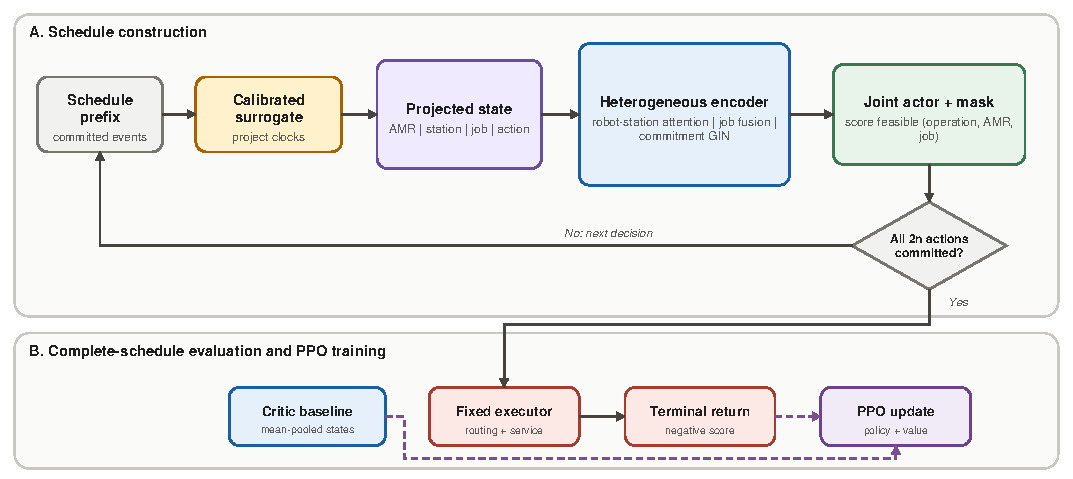
\includegraphics[width=\textwidth]{fig_architecture}
  \caption{Overview of the execution-grounded constructive policy. After each
  feasible operation--AMR--job decision, the completion check either returns
  the updated prefix for another decision or passes the complete schedule to
  the fixed executor. The terminal score and critic baseline provide the
  dashed PPO training inputs.}
  \label{fig:architecture}
\end{figure*}

At each of the $2n$ decision epochs, the policy commits one composite action
$a_t=(\omega,k,j)$ and never revises it. Its \textsc{ExtendGNN} encoder gives
stations their own node type because station occupancy, unlike a fixed travel
matrix, depends on earlier commitments. Station nodes carry projected service
windows $\bm E_t$ and exchange information with robots before jobs are
encoded.

\subsection{Decision State}
\label{sec:arch-state}

Between commitments the state is advanced by the calibrated surrogate
$\hat\Psi$ of Section~\ref{sec:calibration}, not by the executor $\Phi$:
$\Phi$ prices a complete schedule, and running it once per epoch is neither
affordable nor well defined on a prefix. After the prefix $\pi_{1:t}$,
$\hat\Psi$ maintains for each robot $k$ a position $x_k$, a ready time
$\tau_k$, and a class-count vector $N^k$; for each station $d$ an
availability $\alpha_d$ and the list of windows
$E_d^t=\{(\underline{s}_e,\bar{s}_e)\}$ it has already committed; and for each
job $j$ its status (unassigned, carried, delivered) and carrier. The
decision clock is $t_{\mathrm{now}}=\min_k\tau_k$. This bookkeeping is the
concrete form of the tuple $(\bm X_t^A,\bm X_t^J,\bm E_t,\pi_{1:t})$ in
\eqref{eq:state}; the station features $\bm X_t^D$ below are a readout
of $\bm E_t$ at $t_{\mathrm{now}}$.

Table~\ref{tab:features} lists the four feature groups. All channels are
normalised to $[0,1]$ by quantities resolved from the live layout---floor
  extent, the binding suffix cap $\sum_{s\succeq\varsigma}Q_s$ of
  \eqref{eq:nested}, and fleet size. These scales remain fixed across the
  workload study, so changing the number of jobs changes the scheduling
  load rather than the numerical range of the feature channels.

\begin{table}[t]
\caption{Decision-state features.}
\label{tab:features}
\centering
\small
\begin{tabular}{@{}lp{0.60\columnwidth}@{}}
\toprule
Group & Channels \\
\midrule
Robot $\bm x^A_k$ \ (12)
 & busy flag and residual busy time $\tau_k-t_{\mathrm{now}}$; onboard counts
   per class and free nested headroom; jobs currently carried; adjacency
   to a station or waiting cell; distance to the nearest station; local
   robot density within Manhattan radius $2$; position \\[2pt]
Station $\bm x^D_d$ \ (9)
 & inbound/outbound indicator; availability delay
   $(\alpha_d-t_{\mathrm{now}})^+$; committed queue depth, both per robot and
   relative to $|W_d|$ and clipped at one; residual service time of the
   window in progress; total committed workload still outstanding;
   position \\[2pt]
Job $\bm x^J_j$ \ (15)
 & service time $p_j$; time since release; carrier index and status; size
   class $\sigma_j$ one-hot; origin and destination indices; the best-case
   completion time of $j$ over all robots under $\hat\Psi$; origin and
   destination positions \\[2pt]
Action $\bm\phi_t(\omega,k,j)$ \ (3)
 & surrogate travel from $x_k$ to the target station; the downstream
   pickup-to-delivery distance, zero for a delivery; the queueing wait
   $\hat\Psi$ predicts at that station on arrival \\
\bottomrule
\end{tabular}
\end{table}

\subsection{Calibrated Event Surrogate}
\label{sec:calibration}

The surrogate advances only event clocks; it neither reserves grid cells nor
plans paths. For Manhattan distance $d>0$, its calibrated leg time is
\begin{equation}
 \hat t(d)=\max\{d,\;0.891719d+4.492501\}.
 \label{eq:calibrated-travel}
\end{equation}
If a robot is ready at station $q$ at time $r$, its predicted wait is
\begin{align}
 \hat w(q,r)&=(\alpha_q-r)^++\beta_{\min\{z(q,r),3\}},\nonumber\\
 \bm\beta&=(0.317,0.317,2.236,6.415),
 \label{eq:calibrated-wait}
\end{align}
where $z(q,r)$ counts previously committed service windows that end after
$r$. The action arrives after~\eqref{eq:calibrated-travel}, starts after
\eqref{eq:calibrated-wait}, commits a non-preemptive interval of length $p_j$,
and updates the selected robot and station clocks. Thus, projected queue depth
and workload reflect the schedule prefix, but not the executor's eventual
space--time reservations.

We fitted~\eqref{eq:calibrated-travel}--\eqref{eq:calibrated-wait} offline on
159 routable schedules from independently generated instances; one failed
decode was discarded. The corpus supplied 10,280 routed legs. Calibration
reduced travel-time MAE from $2.575$ to $2.179$ ticks and removed the mean
per-leg bias (affine $R^2=0.875$). Queue penalties are bin means of extra wait
beyond station availability, constrained to be nondecreasing with depth. This
small model is used to reduce prefix-construction cost, not as evidence that
the executor has been reproduced; Section~\ref{sec:surrogate-results}
measures the remaining fidelity gap directly.

\subsection{Entity Encoders}
\label{sec:arch-encoders}

Each group is embedded into $\mathbb R^{h}$, $h=128$:
\begin{equation}
 \bm h^A_k=\mathrm{MLP}_A(\bm x^A_k),\quad
 \bm h^D_d=\mathrm{MLP}_D(\bm x^D_d),\quad
 \bm h^J_j=\bm W_J\bm x^J_j ,
 \label{eq:embed}
\end{equation}
collected as $\bm H^A\in\mathbb R^{m\times h}$,
$\bm H^D\in\mathbb R^{|\mathcal D|\times h}$, and
$\bm H^J\in\mathbb R^{n\times h}$, where
$\mathcal D=\mathcal D^{\mathrm{in}}\cup\mathcal D^{\mathrm{out}}$.

\subsection{Robot--Station Interaction}
\label{sec:arch-interaction}

Write $\mathrm{At}(\bm Q,\bm K)=\mathrm{MHA}\big(\mathrm{LN}(\bm Q),
\mathrm{LN}(\bm K),\mathrm{LN}(\bm K)\big)$ for pre-normalised multi-head
attention with four heads. One round couples the two resource types,
\begin{equation}
 \begin{aligned}
 \bm H^D &\leftarrow \bm H^D+\mathrm{At}(\bm H^D,\bm H^A),\\
 \bm H^A &\leftarrow \bm H^A+\mathrm{At}(\bm H^A,\bm H^A),\\
 \bm H^A &\leftarrow \bm H^A+\mathrm{At}(\bm H^A,\bm H^D),
 \end{aligned}
 \label{eq:interaction}
\end{equation}
in that order. Stations first read the approaching fleet, robots exchange
load information, and then read the updated stations. Zero-initialized output
projections make this residual block an identity at the start of training.

\subsection{Job Encoding over the Commitment Graph}
\label{sec:arch-jobs}

Each job fuses the embeddings of the two stations it must visit,
\begin{equation}
 \bm z^{(0)}_j=\bm h^J_j+
 \mathrm{MLP}_F\big([\,\bm h^J_j,\ \bm h^D_{o_j},\ \bm h^D_{d_j}\,]\big).
 \label{eq:fusion}
\end{equation}
The fusion is residual rather than replacing because $|\mathcal D|=10$
station embeddings are shared among $n$ jobs: a replacing fusion writes
what jobs have in common over what distinguishes them.

The prefix induces an undirected graph $\bm A_t$ on jobs. Two jobs are
adjacent if they are consecutive on the same robot, or consecutive at the
same outbound station, in $\pi_{1:t}$; the graph is therefore empty at $t=0$
and accumulates the commitments actually made. Three residual layers of graph
isomorphism convolution refine the embeddings,
\begin{equation}
 \begin{aligned}
 \bm m_j^{(\ell)}&=(1+\epsilon_\ell)\bm z_j^{(\ell-1)}
 +\frac{1}{|\mathcal N_t(j)|}
   \sum_{i\in\mathcal N_t(j)}\bm z_i^{(\ell-1)},\\
 \bm z_j^{(\ell)}&=\bm z_j^{(\ell-1)}+
 \mathrm{LN}\!\left(\mathrm{MLP}_\ell(\bm m_j^{(\ell)})\right),
 \end{aligned}
 \label{eq:gin}
\end{equation}
with $\epsilon_\ell$ learned and $\bm z_j\equiv\bm z^{(3)}_j$. Mean rather
than sum aggregation keeps the message scale stable as $\bm A_t$ densifies
over an episode; the neighbour term is zero when $\mathcal N_t(j)$ is empty.

Only committed sequence arcs enter $\bm A_t$; origin and destination
relationships already enter through the shared station embeddings in
\eqref{eq:fusion}.

\subsection{Composite Actor Head}
\label{sec:arch-actor}

The action is scored jointly rather than factored into a job choice
followed by a robot choice. Let $d(\omega,j)=o_j$ for
$\omega=\textsc{pick}$ and $d(\omega,j)=g_j$ for $\omega=\textsc{del}$, and
let $\bm e_\omega$ be a learned operation embedding. Each candidate triple
receives the logit
\begin{equation}
 \ell_t(\omega,k,j)=\mathrm{MLP}_\pi\big([\,\bm e_\omega,\ \bm h^A_k,\
 \bm z_j,\ \bm h^D_{d(\omega,j)},\ \bm\phi_t(\omega,k,j)\,]\big),
 \label{eq:logit}
\end{equation}
an input of width $4h+3$. The three surrogate channels $\bm\phi_t$ enter
here, at the only place where a robot, a job, and a station are
named together; no pooled embedding can recover the travel and waiting cost
of a specific pairing. Writing $\mathcal A_t$ for the legal set of
Section~\ref{sec:mdp}---pickup only by a robot whose nested rack admits
$\sigma_j$, delivery only by the carrier of $j$---illegal triples are set to
$-\infty$ and
\begin{equation}
 \pi_\theta(a_t\mid s_t)=
 \frac{\exp \ell_t(a_t)}{\sum_{a\in\mathcal A_t}\exp \ell_t(a)} .
 \label{eq:policy}
\end{equation}
Masking guarantees assignment, precedence, and rack feasibility by
construction; remaining decoder failures are recorded by $\nu_\Phi$ in
\eqref{eq:routable-set}.

\subsection{Critic}
\label{sec:arch-critic}

A single value head reads mean-pooled encodings, the job pool taken over
undelivered jobs only:
\begin{equation}
 V_\psi(s_t)=\mathrm{MLP}_V\big([\,\bar{\bm z}_t,\ \bar{\bm h}^A,\
 \bar{\bm h}^D\,]\big).
 \label{eq:critic}
\end{equation}
The actor resolves individual entities, whereas the critic supplies a compact
baseline through three pooled vectors. Its loss also trains the shared
encoder.

\subsection{PPO Training}
\label{sec:training}

A sampled action sequence is decoded to a complete schedule $x$. Let
$S_\Phi(x)$ equal $C_{\max}^{\Phi}(x)$ for a routable schedule and the
executor's finite training score otherwise. In the executor-grounded arms, the
undiscounted terminal return is
\begin{equation}
 R(x)=-S_\Phi(x),
 \label{eq:return}
\end{equation}
while reported makespan excludes failed decodes as specified in
Section~\ref{sec:evaluators}. Because reward is terminal, every prefix has
return-to-go $R(x)$, while the critic gives
step-dependent advantages $\hat A_t=R(x)-V_\psi(s_t)$. PPO maximizes
\begin{align}
 \mathcal L^{\rm clip}
 &=\mathbb E_t\!\left[\min\!\left(r_t\hat A_t,
 \operatorname{clip}(r_t,1-\epsilon,1+\epsilon)\hat A_t\right)\right],
 \label{eq:ppo}
 \\
 r_t&=\pi_\theta(a_t|s_t)/\pi_{\theta_{\rm old}}(a_t|s_t).\nonumber
\end{align}
with a squared value loss. Returns and advantages are normalized over each
batch. Crucially, $\hat\Psi$ still generates every intermediate $s_t$ in both
training and inference; only the complete-schedule cost in~\eqref{eq:return}
comes from $\Phi$. The ideal-objective ablation replaces this cost by
$\widetilde C(x)$ without changing transitions, architecture, or action mask.

\subsection{Cost, Size, and Congestion Channels}
\label{sec:arch-cost}

The encoder costs $O((m+|\mathcal D|)^2h+n^2h)$ per epoch and the joint head
scores at most $2mn$ candidates. The $h=128$ network has 617,605 parameters,
including 49,409 in the value head.

Congestion enters the policy through an identifiable set of channels: the
local robot density in $\bm x^A$, the five occupancy channels of $\bm x^D$
(availability delay, the two queue-depth measures, residual service, and
committed workload), and the predicted wait in $\bm\phi_t$. Everything else
the network sees is geometry, capacity, or workload that an idealized
transport model would also supply. This grouping is what the observability
factor of Section~\ref{sec:experiments} manipulates, and it is why the
factor can be varied without changing capacity: the architecture, its
parameter count, and its action space are identical across the levels.
